\documentclass[journal,12pt,twocolumn]{IEEEtran}

\usepackage{setspace}
\usepackage{gensymb}
\singlespacing
\usepackage[cmex10]{amsmath}

\usepackage{amsthm}

\usepackage{mathrsfs}
\usepackage{txfonts}
\usepackage{stfloats}
\usepackage{bm}
\usepackage{cite}
\usepackage{cases}
\usepackage{subfig}

\usepackage{longtable}
\usepackage{multirow}

\usepackage{enumitem}
\usepackage{mathtools}
\usepackage{steinmetz}
\usepackage{tikz}
\usepackage{circuitikz}
\usepackage{verbatim}
\usepackage{tfrupee}
\usepackage[breaklinks=true]{hyperref}
\usepackage{graphicx}
\usepackage{tkz-euclide}

\usetikzlibrary{calc,math}
\usepackage{listings}
    \usepackage{color}                                            %%
    \usepackage{array}                                            %%
    \usepackage{longtable}                                        %%
    \usepackage{calc}                                             %%
    \usepackage{multirow}                                         %%
    \usepackage{hhline}                                           %%
    \usepackage{ifthen}                                           %%
    \usepackage{lscape}     
\usepackage{multicol}
\usepackage{chngcntr}

\DeclareMathOperator*{\Res}{Res}

\renewcommand\thesection{\arabic{section}}
\renewcommand\thesubsection{\thesection.\arabic{subsection}}
\renewcommand\thesubsubsection{\thesubsection.\arabic{subsubsection}}

\renewcommand\thesectiondis{\arabic{section}}
\renewcommand\thesubsectiondis{\thesectiondis.\arabic{subsection}}
\renewcommand\thesubsubsectiondis{\thesubsectiondis.\arabic{subsubsection}}


\hyphenation{op-tical net-works semi-conduc-tor}
\def\inputGnumericTable{}                                 %%

\lstset{
%language=C,
frame=single, 
breaklines=true,
columns=fullflexible
}
\begin{document}


\newtheorem{theorem}{Theorem}[section]
\newtheorem{problem}{Problem}
\newtheorem{proposition}{Proposition}[section]
\newtheorem{lemma}{Lemma}[section]
\newtheorem{corollary}[theorem]{Corollary}
\newtheorem{example}{Example}[section]
\newtheorem{definition}[problem]{Definition}

\newcommand{\BEQA}{\begin{eqnarray}}
\newcommand{\EEQA}{\end{eqnarray}}
\newcommand{\define}{\stackrel{\triangle}{=}}
\bibliographystyle{IEEEtran}
\raggedbottom
\setlength{\parindent}{0pt}
\providecommand{\mbf}{\mathbf}
\providecommand{\pr}[1]{\ensuremath{\Pr\left(#1\right)}}
\providecommand{\qfunc}[1]{\ensuremath{Q\left(#1\right)}}
\providecommand{\sbrak}[1]{\ensuremath{{}\left[#1\right]}}
\providecommand{\lsbrak}[1]{\ensuremath{{}\left[#1\right.}}
\providecommand{\rsbrak}[1]{\ensuremath{{}\left.#1\right]}}
\providecommand{\brak}[1]{\ensuremath{\left(#1\right)}}
\providecommand{\lbrak}[1]{\ensuremath{\left(#1\right.}}
\providecommand{\rbrak}[1]{\ensuremath{\left.#1\right)}}
\providecommand{\cbrak}[1]{\ensuremath{\left\{#1\right\}}}
\providecommand{\lcbrak}[1]{\ensuremath{\left\{#1\right.}}
\providecommand{\rcbrak}[1]{\ensuremath{\left.#1\right\}}}
\theoremstyle{remark}
\newtheorem{rem}{Remark}
\newcommand{\sgn}{\mathop{\mathrm{sgn}}}
%\providecommand{\res}[1]{\Res\displaylimits_{#1}} 
%\providecommand{\norm}[1]{\left\lVert#1\right\rVert}
\providecommand{\norm}[1]{\lVert#1\rVert}
\providecommand{\mtx}[1]{\mathbf{#1}}
%\providecommand{\mean}[1]{E\left[ #1 \right]}
\providecommand{\fourier}{\overset{\mathcal{F}}{ \rightleftharpoons}}
%\providecommand{\hilbert}{\overset{\mathcal{H}}{ \rightleftharpoons}}
\providecommand{\system}{\overset{\mathcal{H}}{ \longleftrightarrow}}
	%\newcommand{\solution}[2]{\textbf{Solution:}{#1}}
\newcommand{\solution}{\noindent \textbf{Solution: }}
\newcommand{\cosec}{\,\text{cosec}\,}
\providecommand{\dec}[2]{\ensuremath{\overset{#1}{\underset{#2}{\gtrless}}}}
\newcommand{\myvec}[1]{\ensuremath{\begin{pmatrix}#1\end{pmatrix}}}
\newcommand{\mydet}[1]{\ensuremath{\begin{vmatrix}#1\end{vmatrix}}}
\numberwithin{equation}{subsection}
\makeatletter
\@addtoreset{figure}{problem}
\makeatother
\let\StandardTheFigure\thefigure
\let\vec\mathbf
\renewcommand{\thefigure}{\theproblem}
\def\putbox#1#2#3{\makebox[0in][l]{\makebox[#1][l]{}\raisebox{\baselineskip}[0in][0in]{\raisebox{#2}[0in][0in]{#3}}}}
     \def\rightbox#1{\makebox[0in][r]{#1}}
     \def\centbox#1{\makebox[0in]{#1}}
     \def\topbox#1{\raisebox{-\baselineskip}[0in][0in]{#1}}
     \def\midbox#1{\raisebox{-0.5\baselineskip}[0in][0in]{#1}}
\vspace{3cm}
\title{EE3025-Assignment 1}
\author{C Shruti - EE18BTECH11006}
\maketitle
\newpage
\bigskip
\renewcommand{\thefigure}{\theenumi}
\renewcommand{\thetable}{\theenumi}
Download all python codes from 
\begin{lstlisting}
https://github.com/shruti-chepuri/EE3025/blob/main/Assignment_1/codes
\end{lstlisting}
%
and latex-tikz codes from 
%
\begin{lstlisting}
https://github.com/shruti-chepuri/EE3025/tree/main/Assignment_1
\end{lstlisting}
(5.3) The system h(n) is said to be stable if 
\begin{align}
\sum_{n=-\infty}^{\infty}{|h(n)|} < \infty
\end{align}
Is the system defined by (3.2) stable for impulse response in (5.1)?
\section{Solution}
Given system: 
\begin{align}
\label{eq:system}
y(n)+\frac{1}{2}y(n-1) = x(n)+x(n-2) \\
y(n)=0 \text{ for }y<0
\end{align}
Applying Z-transform:
\begin{align}
Y(z) + \frac{1}{2}z^{-1}Y(z)=X(z) + z^{-2}X(z)\\
Y(z)=\frac{2(z^2+1)}{z(2z+1)}X(z)
\end{align}
Finding H(z):
\begin{align}
H(z) = \frac{Y(z)}{X(z)}\\
H(z) = \frac{2(z^2+1)}{z(2z+1)} \\
H(z) = \frac{1+z^{-2}}{1+\frac{1}{2}z^{-1}}
\end{align}
Impulse response of this system(h(n)):
\begin{align}
    h(n)= Z^{-1}(\frac{1}{1+\frac{1}{2}z^{-1}} + \frac{z^{-2}}{1+\frac{1}{2}z^{-1}})\\
    h(n)=(\frac{-1}{2})^nu(n) + (\frac{-1}{2})^{n-2}u(n-2)
\end{align}
Given stability criteria :
\begin{align}
\sum_{n=-\infty}^{\infty}{|h(n)|} < \infty
\end{align}
Substituting h(n) we have,
\begin{align}
\sum_{n=-\infty}^{\infty}{|(\frac{-1}{2})^nu(n) + (\frac{-1}{2})^{n-2}u(n-2)|} < \infty \\
\sum_{n=-\infty}^{\infty}{|(\frac{1}{2})^nu(n) + (\frac{1}{2})^{n-2}u(n-2)|} < \infty \\
2\sum_{n=-\infty}^{\infty}{|(\frac{1}{2})^nu(n)|} < \infty \\
2(\frac{1}{1-\frac{1}{2}}) = 4 < \infty
\end{align}
So, the system is stable.\\
Verification in Z plane:\\ 
When h(n) is bounded i.e
\begin{align}
\sum_{n=-\infty}^{\infty} |h(n)|  &< \infty \\
\sum_{n=-\infty}^{\infty}|h(n)z^{-n}|_{|z|=1}&<\infty \\
\sum_{n=-\infty}^{\infty}|h(n)z^{-n}|_{|z|=1}&<|\sum_{n=-\infty}^{\infty}h(n)z^{-n}|_{|z|=1} \\
\implies |H(z)|_{|z|=1}&<\infty 
\end{align}
from triangle inequality. This shows us that the unit circle should lie in the ROC for the system to be stable. Now,
\begin{align}
H(z) = \frac{2(z^2+1)}{z(2z+1)} \\
Poles = 0 , -\frac{1}{2} \\
Zeros = +1j, -1j
\end{align}
\begin{figure}[h!]
    \centering
    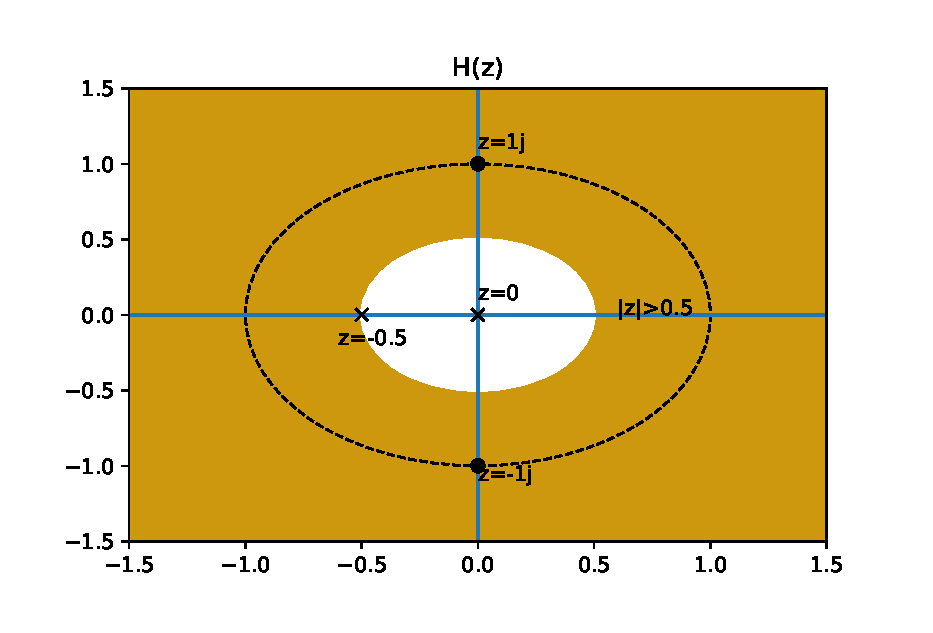
\includegraphics[width=10 cm]{EE3025/Assignment_1/figs/z_plane.eps}
    \caption{Unit circle lies in ROC}
    \label{zn}
\end{figure} \\
Hence from the Z plane plot the system is stable.\\
Verification:\\
BIBO Stability : For a given system and for every bounded input, if the output is bounded then it is stable. 
For a system to be stable the output should be bounded for every bounded input.(BIBO stability).
Consider a bounded input sequence x(n) 
\begin{align}
\abs{x(n)}<B_x(finite)
\end{align}
Then by using the convolution property,
\begin{align}
 |y(n)|= |\sum_{-\infty}^{\infty}h(k)x(n-k)|\\
 |y(n)| \leq B_x\sum_{-\infty}^{\infty}|h(k)|
\end{align}
 This holds only if
\begin{align}
\sum_{-\infty}^{\infty}|{h(n)}| < 
\infty \\
\text{then we have} |{y(n)}| \leq B_y < \infty 
\end{align}
Thus the output is bounded for bounded input if the impulse response is absolutely summable.\\
Verification:- Given bounded input x(n).,
\begin{align}
x(n) = \cbrak{1,1,2,4,3,1}\\
y(n)+\frac{1}{2}y(n-1) = x(n)+x(n-2)
\end{align} \\
\begin{figure}[h!]
    \centering
    \includegraphics[width=10cm]{EE3025/Assignment_1/figs/x_n.eps}
    \caption{Given input}
    \label{xn}
\end{figure}
x(n) is bounded.\\
\begin{figure}[h!]
    \centering
    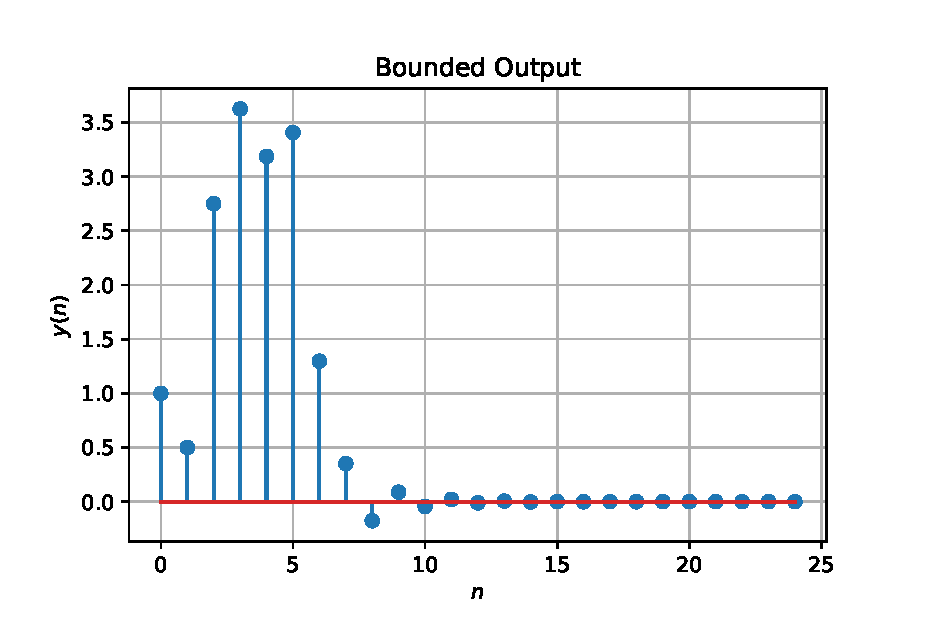
\includegraphics[width=10cm]{EE3025/Assignment_1/figs/y_n.eps}
    \caption{Bounded output}
    \label{yn}
\end{figure} \\
The system returns bounded output for the given bounded input. Implies, the system is stable.\\ 
\end{document}
